\documentclass[12pt]{beamer}

\usepackage{subfigure}
\usepackage{caption}
\usepackage{graphicx}
%\usepackage{natbib}
%\usepackage{bibentry}
\usepackage{biblatex}

\bibliography{refs}

\mode<presentation>
\subtitle{M. Lazaro-Gredilla, J. Quinonero-Candela, C. E. Rasmussen, \
A. R. Figueiras-Vidali 2010, \emph{Journal of Machine Learning Research 11}, pp 1865-1881}
\title{Sparse Spectrum Gaussian Process Regression}
\date{}
\author{Peter Ashwell}

%\newcommand{\newblock}{}

\begin{document}
\maketitle

\begin{frame}
	\frametitle{Astroinformatics and Transients}
	\begin{figure}
	  \centering
	  \subfigure {	
	  	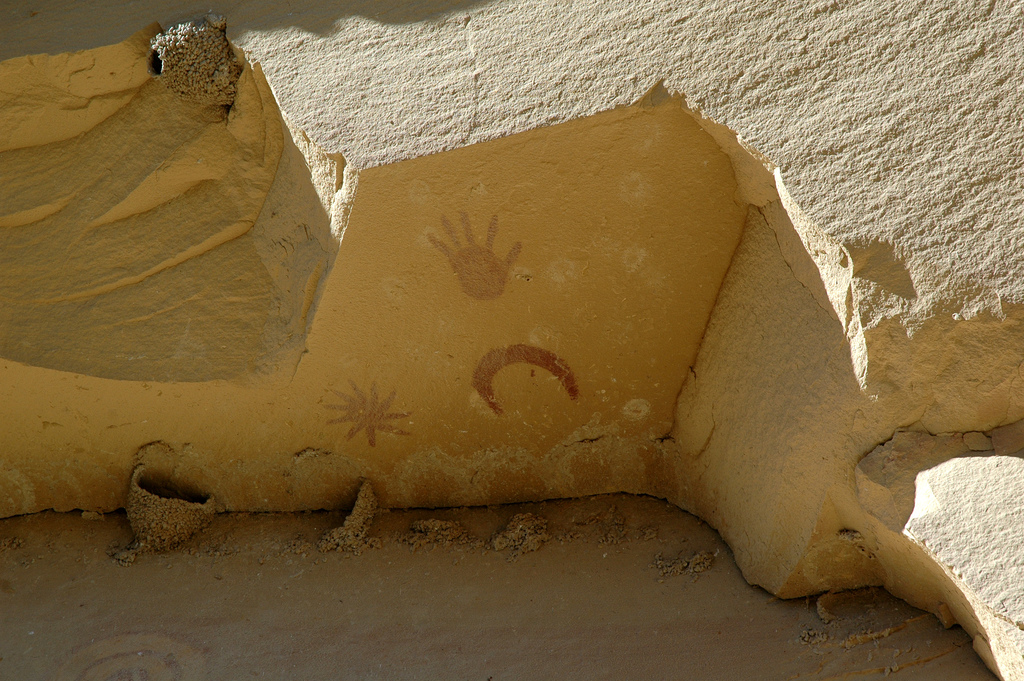
\includegraphics[width=140px]{ccs.jpg}
	  }
	  \subfigure {
	  	\includegraphics[width=140px]{askap.png}
	  }
  	%\caption{Wall painting in Chaco Canyon, NM USA}
	\end{figure}
	The ultimate goal of Astroinformatics is the automatic analysis of large amounts of telescope data. This will help astronomers to do research on interesting events in our universe.

\end{frame}

\begin{frame}
	\frametitle{Time Series Analysis and Gaussian Processes (GPs)}
	\begin{figure}
		\subfigure[Time series of supernova] {
				\captionsetup[subfigure]{labelformat=empty}

			\includegraphics[width=140px]{sne.jpg}
		 }
		\subfigure[GP learning sinc function] {
				\captionsetup[subfigure]{labelformat=empty}

		  	\includegraphics[width=130px]{gp.PNG}
		}
		\captionsetup[subfigure]{labelformat=empty}
	\end{figure}
  Gaussian process: Given some observed mappings from an unknown function $f$: $x \mapsto y$, make predictions about $f$ at unobserved $x_{u}$, or, tell me if some set of other observations were likely to come from $f$.
\end{frame}

\begin{frame}
	\frametitle{Previous Work and the Paper}
	Gaussian processes are computationally and space expensive, both for training and prediction - for $n$ training points:

	\begin{table}
	  \begin{footnotesize}
	  \begin{center}
	  \begin{tabular}{llll}
		Author & Space & Time \\
		Theory, O'Hagan ~\cite{o1978curve} 1978 & - & - \\
		Rasmussen and Williams ~\cite{rasmussen2006gpfml} 2006 & $O(n^{3})$ & $O(n^{2})$ \\
		Various 2001 - 2008  \cite{snelson2005sgppi} \cite{tresp2000bcm} \cite{walder2008sparse} & $O(nm^{2})$ & train $O(nm)$ predict $O(m^{2})$  \\
		This Paper 2010& $O(nm^{2})$ & train $O(nm)$ predict $O(m^{2})$ \\
	  \end{tabular}
	  \end{center}
	  \end{footnotesize}
	\end{table}
	Where $m << n$, $m$ is the number of basis functions in sparse approximation.
	\begin{tiny}
	\begin{enumerate}
		\item \fullcite{o1978curve}
		\item \fullcite{rasmussen2006gpfml}
		\item \fullcite{tresp2000bcm}
		\item \fullcite{snelson2005sgppi}
		\item \fullcite{walder2008sparse}
	\end{enumerate}
	\end{tiny}
\end{frame}

\begin{frame}
  \frametitle{Method}
  \begin{figure}
  	\def \svgwidth{0.85\columnwidth}
  	\input{gproc_fin.pdf_tex}
  \end{figure}
  \begin{tiny}
  \begin{enumerate}
  	\item[6.] A. B. Carlson. Communication Systems. McGraw-Hill, 3rd edition, 1986.
	\item[7.] M. L. Stein. Interpolation of Spatial Data. Springer Verlag, 1999.
  \end{enumerate}
  \end{tiny}
\end{frame}

\begin{frame}
	\frametitle{Paper results and review}
	\begin{itemize}
		\item Evaluation shows slight improvement in accuracy over other sparse methods
		\item Small sacrifice in accuracy over full $O(n^{3})$ GP
		\item More vulnerable than other GP methods to overfitting
	\end{itemize}
	\begin{figure}
	\subfigure{
		\includegraphics[width=150px]{eval3.PNG}
	}
	\end{figure}
\end{frame}

\begin{frame}
  \frametitle{Paper results and review}
		\begin{itemize}
			\item Attractive theoretical computational bounds $O(m^{2})$ for large amounts of data analysis
			\item Respected, well cited experts in GP field and published in highly ranked journal
			\item Evaluation does not discuss exact run-times compared to other sparse methods
			\item Otherwise, rigorous evaluation shows an effective tool for multi-dimensional data modelling
		\end{itemize}
\end{frame}

\begin{frame}
	\frametitle{In the Context of my Project}
	This is a practical approach to modelling light curves for large volumes of data, however:
	\begin{itemize}
	  \item There may be faster or more accurate methods 
	\item May not be suitable for modelling astronomical data (overfitting risk)
	\item This approach was not evaluated in terms of predictive power, just fit accuracy
	\end{itemize}
	My research approach is as follows:
	\begin{enumerate}
	  \item Simulate astronomical data 
	  \item Decide on a method to rapidly identify transients, with confidence (perhaps this approach)
	  \item Implement and evaluate method using simulated data
	  \item Expand implementation to large data streams if possible
	\end{enumerate}
%	\cite{tresp2000bcm}
\end{frame}

	
%\bibliography{refs}{}
%\bibliographystyle{plain}
\end{document}
